
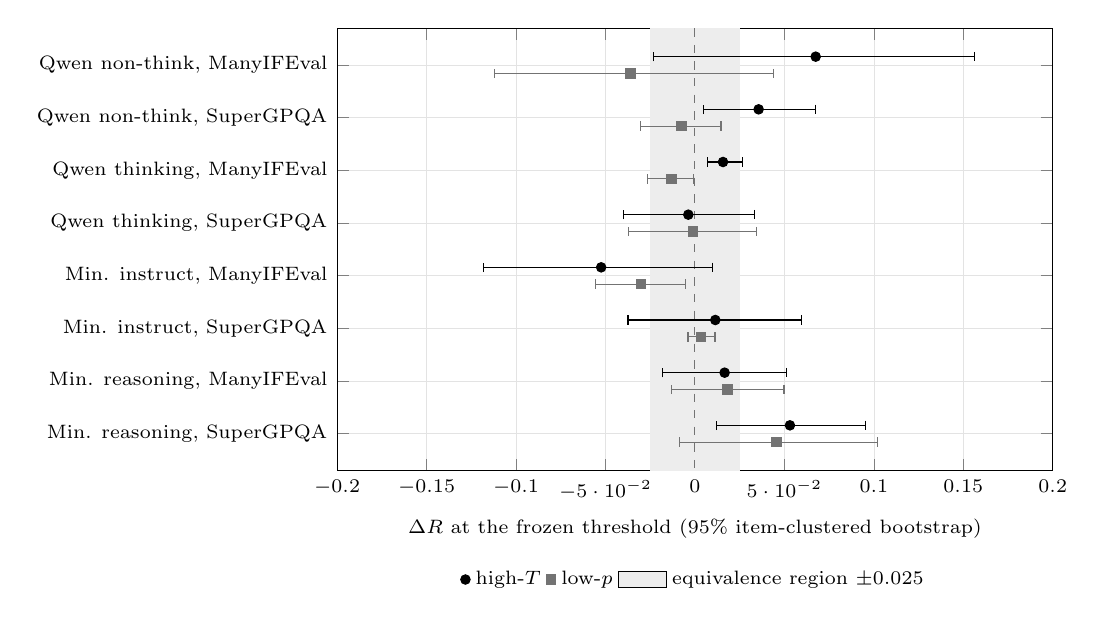
\begin{tikzpicture}
\begin{axis}[
  width=0.88\textwidth, height=7.2cm,
  ytick={0,1,2,3,4,5,6,7}, yticklabels={{Qwen non-think, ManyIFEval},{Qwen non-think, SuperGPQA},{Qwen thinking, ManyIFEval},{Qwen thinking, SuperGPQA},{Min. instruct, ManyIFEval},{Min. instruct, SuperGPQA},{Min. reasoning, ManyIFEval},{Min. reasoning, SuperGPQA}}, y dir=reverse,
  ymin=-0.7, ymax=7.7,
  xmin=-0.20, xmax=0.20,
  xlabel={$\Delta R$ at the frozen threshold (95\% item-clustered bootstrap)},
  tick label style={font=\scriptsize}, label style={font=\scriptsize},
  legend style={font=\scriptsize, at={(0.5,-0.20)}, anchor=north, legend columns=3, draw=none},
  grid=major, grid style={gray!22,very thin}]
\fill[black!7] (axis cs:-0.025,-0.7) rectangle (axis cs:0.025,7.7);
\draw[black!55,dashed] (axis cs:0,-0.7) -- (axis cs:0,7.7);
\addplot[only marks, mark=*, mark size=1.7pt, color=black,
  error bars/.cd, x dir=both, x explicit, error bar style={black}]
  coordinates {(0.0675,-0.16) += (0.0889,0) -= (0.0908,0) (0.0356,0.84) += (0.0318,0) -= (0.0308,0) (0.0157,1.84) += (0.0108,0) -= (0.0088,0) (-0.0037,2.84) += (0.0368,0) -= (0.0363,0) (-0.0524,3.84) += (0.0620,0) -= (0.0660,0) (0.0114,4.84) += (0.0480,0) -= (0.0488,0) (0.0166,5.84) += (0.0344,0) -= (0.0346,0) (0.0531,6.84) += (0.0424,0) -= (0.0411,0)};
\addlegendentry{high-$T$}
\addplot[only marks, mark=square*, mark size=1.7pt, color=black!55,
  error bars/.cd, x dir=both, x explicit, error bar style={black!55}]
  coordinates {(-0.0361,0.16) += (0.0799,0) -= (0.0757,0) (-0.0076,1.16) += (0.0222,0) -= (0.0228,0) (-0.0132,2.16) += (0.0123,0) -= (0.0133,0) (-0.0011,3.16) += (0.0356,0) -= (0.0359,0) (-0.0302,4.16) += (0.0248,0) -= (0.0256,0) (0.0035,5.16) += (0.0077,0) -= (0.0074,0) (0.0183,6.16) += (0.0315,0) -= (0.0315,0) (0.0455,7.16) += (0.0563,0) -= (0.0540,0)};
\addlegendentry{low-$p$}
\addlegendimage{area legend, fill=black!7, draw=none}
\addlegendentry{equivalence region $\pm0.025$}
\end{axis}
\end{tikzpicture}
